\begin{figure*}[t!]
    \centering
    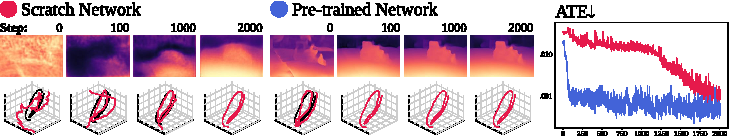
\includegraphics[width=\linewidth]{figures/init_vs_pretrain_pdf.pdf}
    \caption{\textbf{Effects of pretraining.} While a randomly initialized FlowMap network often provides accurate poses after optimization, pre-training leads to faster convergence and slightly improved poses. Here we plot depth estimates at specific optimization steps (left) as well as pose accuracy with respect to COLMAP during optimization (right). Randomly initialized FlowMap networks often require more than 20,000 steps to match the accuracy of a pre-trained initialization at 2,000 steps.}
    \label{fig:prior}
\end{figure*}
